\section{Results}

\begin{frame}{The energy of the modes for each $\lambda$}
	\begin{figure}[h]
		\centering
		\caption{$\omega_1$ as a function of $\lambda$ for the massless case in the \textbf{external field approximation}.}
		\label{fig:figures-eigenvalue_evolution_a_1_0-png}
		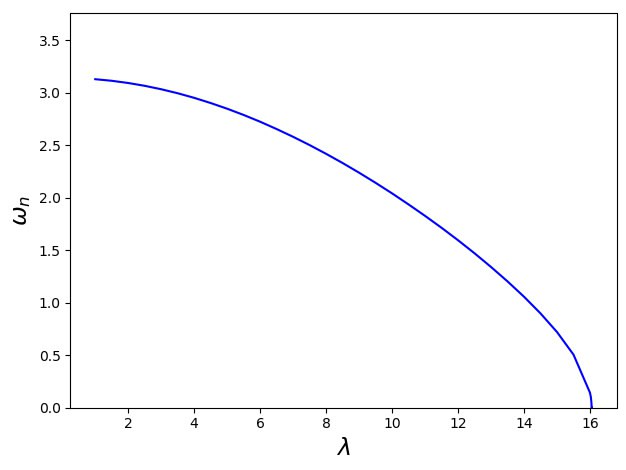
\includegraphics[width=0.6\textwidth]{figures/eigenvalues-external-field-approximation.png}
	\end{figure}
\end{frame}

\begin{frame}{The energy of the modes for each $\lambda$}
\begin{figure}[h]
	\centering
	\caption{$\omega_1$ as a function of $\lambda$ in the mode sum prescription with $N=1$. }
	\label{fig:figures-eigenvalues_ambjorn}
	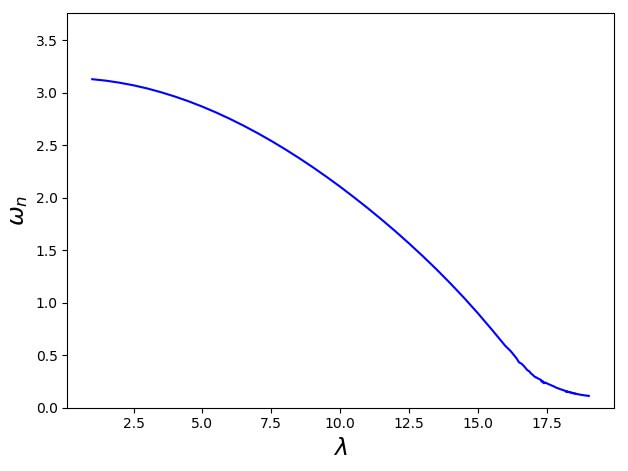
\includegraphics[width=0.6\textwidth]{figures/eigenvalues_ambjorn.png}
\end{figure}
\end{frame}

\begin{frame}{The energy of the modes for each $\lambda$}
\begin{figure}[h]
	\centering
	\caption{The energy of the first three modes of the scalar field in the Hadamard point-splitting prescription with cutoff $N=12$ as $\lambda$ increases.}
	\label{fig:figures-eigenvalue-evolution-png}
	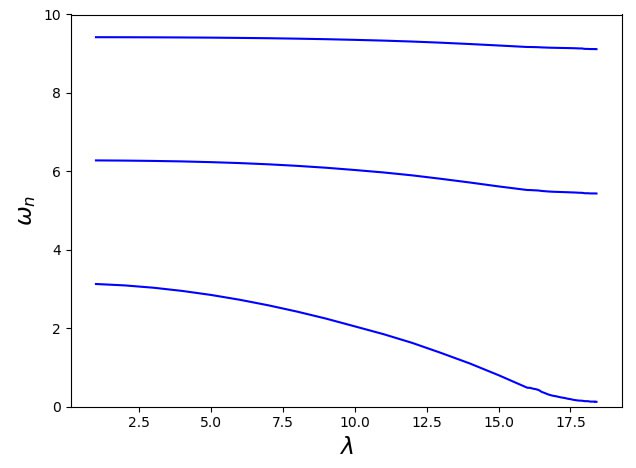
\includegraphics[width=0.5\textwidth]{figures/eigenvalue-evolution.png}
	
\end{figure}
\end{frame}
\begin{frame}{The energy of the modes at each $\lambda$}
\begin{figure}[h]
	\centering
	\caption{$\omega_1$ as a function of $\lambda$ for the \textcolor{blue}{mode sum formula prescription}, \textcolor{orange}{Hadamard point-splitting prescription} and \textcolor{green}{external field approximation}.}
	\label{fig:figures-eigenvalue-evolution-png}
	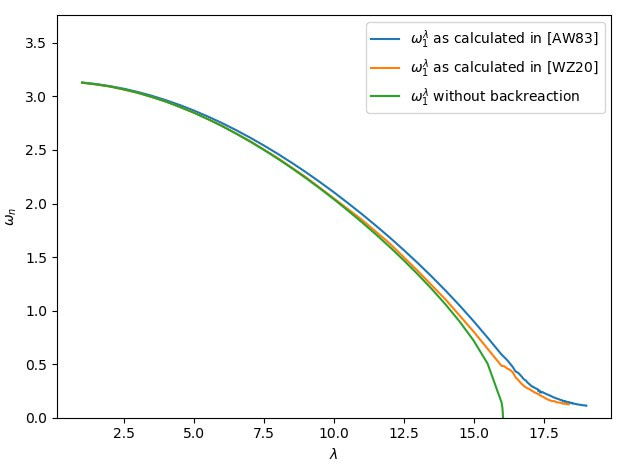
\includegraphics[width=0.5\textwidth]{figures/comparing-energies.png}
	
\end{figure}
\end{frame}


\begin{frame}{Self consistent vacuum polarizations for low $\lambda$}
	\begin{columns}
	    \begin{column}{0.5\textwidth}
	    \begin{figure}[h]
	    	\centering
	    	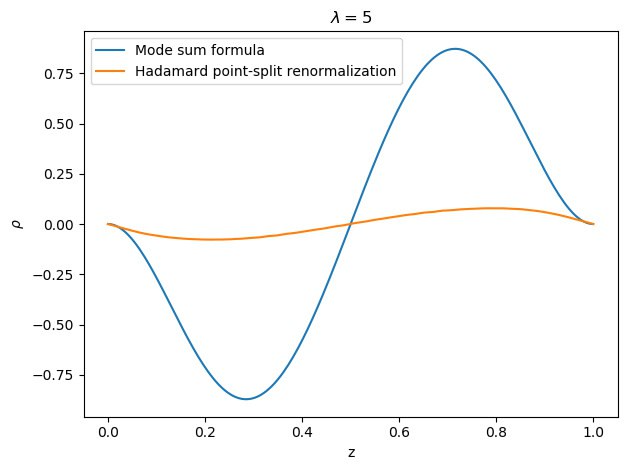
\includegraphics[width=0.8\textwidth]{figures/low-lambda-vacuum-polarization.png}
	    	\caption{$\lambda=5$ comparison of the self consistent vacuum polarization.}
	    	\label{fig:figures-}
	    \end{figure}
	    \end{column}
	    \begin{column}{0.5\textwidth}
	    \begin{figure}[h]
	    	\centering
	    	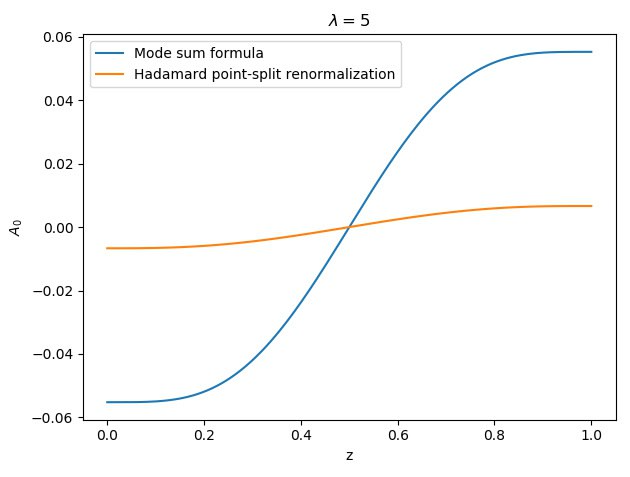
\includegraphics[width=0.8\textwidth]{figures/low-lambda-induced-A0.png}
	    	\caption{$\lambda=5$ comparison of the self consistent induced $A_0$}
	    	\label{fig:figures-}
	    \end{figure}
	    \end{column}
	\end{columns}
\end{frame}
\begin{frame}{Self consistent vacuum polarizations for high $\lambda$}
	\begin{columns}
	    \begin{column}{0.5\textwidth}
	    \begin{figure}[h]
	    	\centering
	    	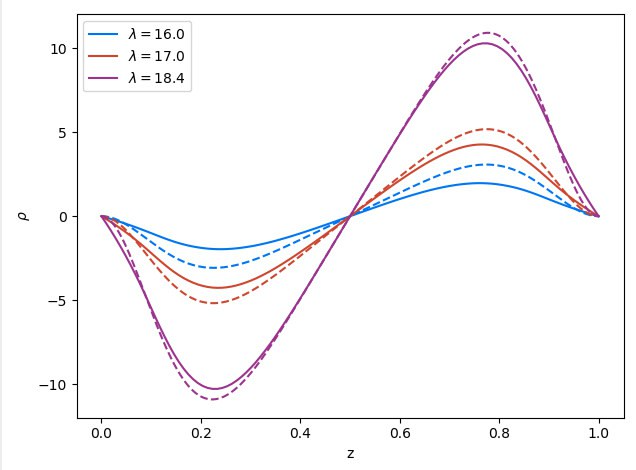
\includegraphics[width=0.8\textwidth]{figures/high-lambda-vacuum-polarization.png}
	    	\caption{Higher values of $\lambda$ comparison of the self consistent vacuum polarization.}
	    	\label{fig:figures-}
	    \end{figure}
	    \end{column}
	    \begin{column}{0.5\textwidth}
	    \begin{figure}[h]
	    	\centering
	    	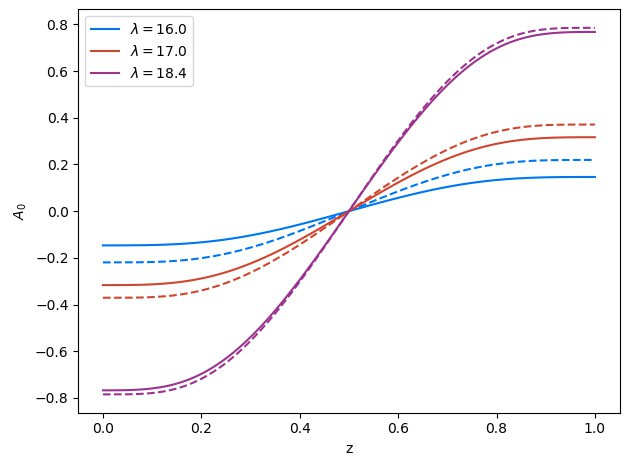
\includegraphics[width=0.8\textwidth]{figures/high-lambda-induced-A0.png}
	    	\caption{Higher values of $\lambda$ comparison of the self consistent vacuum polarization.}
	    	\label{fig:figures-}
	    \end{figure}
	    \end{column}
	\end{columns}
	Dashed lines: mode sum formula. 

	Solid lines: Hadamard point-splitting renormalization.
\end{frame}

\begin{frame}{Vacuum polarization for different $\lambda$}
	\begin{figure}[h]
		\centering
		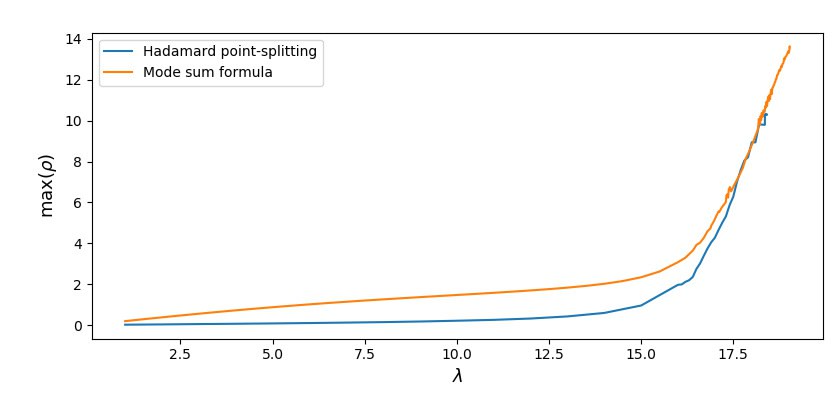
\includegraphics[width=0.8\textwidth]{figures/different-lambda-rho.png}
		\caption{The maximum of the vacuum polarization for different values of the background electric field strength.}
		\label{fig:figures-different-lambda-rho-png}
	\end{figure}
\end{frame}
